\chapter{TikZ 绘图初步}

PGF ("portable graphics format") is the basic layer, providing a set of basic commands for producing graphics, and TikZ ("TikZ ist kein Zeichenprogramm" (German) or "TikZ is not a Drawing program") is the frontend layer with a special syntax, making the use of PGF easier. TikZ commands are prevalently similar to Metafont, the option mechanism is similar to PsTricks syntax. 
本章内容主要参考:\cite{WIKIBOOKS}.

\section{基本使用}

TikZ 可以直接在 .tex 文件中使用,也可以使用 TikZ 生产独立的图像文件,其模版如下:

\begin{minted}{latex}
\documentclass{standalone}
\usepackage{tikz}
\usetikzlibrary{<list of libraries separated by commas>}

\begin{document}

\begin{tikzpicture}[<options>]
  <environment contents>
\end{tikzpicture}

\end{document}
\end{minted}

\begin{remark*}
  每条绘图命令必须以分号结束。
\end{remark*}

先看一个简单的例子:

\inputminted{latex}{examples/tikz/preliminaries/standalone-example.tex}

生成的图像文件:

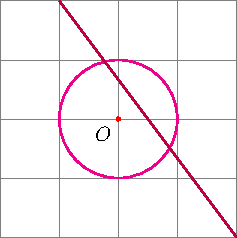
\includegraphics{examples/tikz/preliminaries/standalone-example.pdf}

\subsection{行内模式:\protect\verbum*{tikz} 命令}

\mint{latex}|\tikz[<options>]{<path commands>}|

One special option for this case is \mintinline{latex}{baseline = <dimension>}. Without that option the lower end of the picture is put on the baseline of the surrounding text. Using this option, you can specify that the picture should be raised or lowered such that the height \verbum{<dimension>} is on the baseline.

下面的代码演示了行内 TikZ 绘图效果:

\begin{texcode}
我们可以直接在行内绘制图形,如:直线\tikz \draw (0,0) -- (2em,1em);(注意
命令之后必须要以分号结束)。当不指定 baseline 参数时,图形的下端将与文本下端平齐,
当指定 baseline 参数时,图形的原点将定位到指定的高度,如:
\tikz{
  \draw (0,0) circle (1em); 
  \draw (0,0) rectangle (1em,1em);
}
\tikz[baseline=2em]{
  \draw (0,0) circle (1em); 
  \draw (0,0) rectangle (1em,1em);
}
\tikz[baseline=-3em]{
  \draw (0,0) circle (1em); 
  \draw (0,0) rectangle (1em,1em);
}
\end{texcode}

\subsection{\protect\verbum{tikzpicture} 环境}

\begin{minted}{latex}
\begin{tikzpicture}[<options>]
  <tikz commands>
\end{tikzpicture}
\end{minted}

例如绘制坐标轴:

\begin{texcode}
\begin{tikzpicture}[scale=.75]
  \draw[help lines] (-2,-2) grid (2,2);
  \draw[-latex] (-3,0) -- (3,0) node[below right] {$x$};
  \draw[-latex] (0,-3) -- (0,3) node[above left] {$y$};
  \node[below left] at (0,0) {$O$};
\end{tikzpicture}
\end{texcode}

\section{坐标系}

Coordinates are specified in round brackets in an arbitrary TEX dimension either using Cartesian coordinates (comma separated), e.g. 1cm in the x direction and 2pt in the y direction

\begin{table}[!h]
\begin{center}
\caption{TikZ 坐标}
\begin{tabular}{ccc}
  \toprule
  Coordinate type	& Syntax & Example\\
  \midrule
  Cartesian	& (x,y)	& (1cm,2pt)\\
  Polar	& (theta:radius) & (30:1cm)\\
  Relative to last position	& ++(x,y)	& ++(2cm,2cm)\\
  \bottomrule
\end{tabular}
\end{center}
\end{table}

\section{路径 Path}

A path is a series of straight and curved line segments (in a simplified explanation). The instruction has to end with a semicolon.

\mint{latex}|\path[<options>]⟨specification⟩;|

One instruction can spread over several lines, or several instructions can be put on one line.

\subsection{Path actions}

Options for path actions are e.g: \verbum{draw}, \verbum{fill}, \verbum{pattern}, \verbum{shade}, \verbum{clip}, \verbum{use as bounding box}. These may be used as following

\begin{minted}{latex}
\path[draw]             % Draw the line/curve 
\path[fill]             % Fill the area under the curve
\path[fill,draw]        % Fill as well as draw the lines (borders)
\path[pattern]          % 
\path[shade]            % a variation on filling that changes colors smoothly from one to another
\path[shade,draw]       % shade as well as draw 
\path[clip]             % all subsequent drawings up to the end of the current scope are clipped against the current path and the size of subsequent paths will not be important for the picture size 
\path[use as bounding box]
\end{minted}

Above command can also be written equivalently as \verbum*{draw}, \verbum*{fill}, \verbum*{filldraw}, \verbum*{pattern}, \verbum*{shade}, \verbum*{shadedraw}, \verbum*{clip}, \verbum*{useasboundingbox}. These commands are explained in details in subsequent section.

\subsection{Geometric path actions}

Geometric path options: \verbum{rotate=<angle in degree>}, \verbum{xshift=<length>}, \verbum{yshift=<length>}, \verbum{scale=<factor>}, \verbum{xscale=<factor>}, \verbum{yscale=<factor>}.

\subsection{Color and opacity}

The most common way is to specify just the color name or \verbum{color=<color name>}. In this case it will color the boarders/area according to the command (\verbum*{draw},\verbum*{fill}) used.

There can be different elements in a drawing so it may require specifying them separately for which one may use

\verbum{draw=<line color>}, \verbum{draw opacity=<factor>}

\verbum{fill=<fill color>}, \verbum{fill opacity=<factor>}

\verbum{text=<text color>}, \verbum{text opacity=<factor>}

\verbum{pattern color=<color>},

\dots

Predefined colors: red, green, blue, cyan, magenta, yellow, black, gray, darkgray, lightgray, brown, lime, olive, orange, pink, purple, teal, violet and white.

The opacity factor values can be in range of 0 (=fully transparent) to 1 (=fully opaque).

\subsection{Line width}

Line width options: \verbum{line width=<dimension>}, and abbreviations \verbum{ultra thin} for 0.1pt, \verbum{very thin} for 0.2pt, \verbum{thin} for 0.4pt (the default width), \verbum{semithick} for 0.6pt, \verbum{thick} for 0.8pt, \verbum{very thick} for 1.2pt, \verbum{ultra thick} for 1.6pt.

\subsection{Line end}

Line end, line join options: 

\verbum{line cap=<type: round, rect, or butt>}, 

\verbum{arrows=<start arrow kind>-<end arrow kind>}, 

\verbum{rounded corners", "rounded corners=<size>}, 

\verbum{line join=<type: round, bevel, or miter>}.

\subsection{Line pattern}

Line pattern options: 

\verbum{dash pattern=<dash pattern>} (e.g. \verbum{dash pattern=on 2pt off 3pt on 4pt off 4pt}), 

\verbum{dash phase=⟨dash phase⟩}, 

\verbum{solid}, 

\verbum{dashed}, 

\verbum{dotted}, 

\verbum{dashdotted}, 

\verbum{densely dotted}, 

\verbum{loosely dotted}, 

\verbum{double}.

Options for filling paths are e.g. 

\verbum{fill=<fill color>}, 

\verbum{pattern=<name>}, 

\verbum{pattern color=<color>}

\section{\protect\verbum*{draw}}

\subsection{直线}

\begin{texcode}[color={}]
\tikz \draw (1,0) -- (0,0) -- (0,1);
\end{texcode}

\begin{texcode}[color={}]
\tikz \draw (1,0) -- (0,0) -- (0,1) -- cycle;
\end{texcode}

\begin{texcode}[color={}]
\tikz \draw (0,0) -- (2,0) (0,1) -- (2,1);
\end{texcode}

\begin{texcode}[color={}]
\tikz \draw (0,0) -| (1,1);%先水平, 后垂直
\end{texcode}

\begin{texcode}[color={}]
\tikz \draw (0,0) |- (1,1);%先垂直, 后水平
\end{texcode}

\subsection{曲线}

\begin{texcode}[color={}]
% Bezier curve
\tikz \draw (0,0) .. controls (1,1) .. (4,0)
            (5,0) .. controls (6,0) and (6,1) .. (5,2);
\end{texcode}

\begin{texcode}[color={}]
\begin{tikzpicture}
  \draw (0,0) to (3,2);
  \draw (0,0) to[out=90,in=180] (3,2);
  \draw (0,0) to[bend right] (3,2);
\end{tikzpicture}
\end{texcode}

\subsection{Rectangle}

\begin{texcode}[color={}]
\tikz \draw (0,0) rectangle (2,3);
\end{texcode}

\subsection{Circle \& Ellipse}

\begin{texcode}[color={}]
\begin{tikzpicture}
  %\draw (0,0) circle [radius=1.5];
  \draw (0,0) circle (2cm); % old syntax with round brackets instead of square brackets
  %\draw (0,0) circle [x radius=1.5cm, y radius=10mm];
  %\draw (0,0) circle (1.2cm and 8mm); % old syntax
  %\draw (0,0) circle [x radius=1cm, y radius=5mm, rotate=30];
  %\draw[rotate=30] (0,0) ellipse (20pt and 10pt);  % old syntax
\end{tikzpicture}
\end{texcode}

\subsection{Arc}

\begin{texcode}[color={}]
\begin{tikzpicture}
  \draw (0,0)  arc[radius = 8mm, start angle= 0, end angle= 270];
  \draw (0,0)  arc[x radius = 1.75cm, y radius = 1cm, start angle= 0, end angle= 315];
\end{tikzpicture}
\end{texcode}

\subsection{Parabola, Sine and Cosine curve}

\begin{texcode}[color={}]
\begin{tikzpicture}
  \draw[help lines] (0,0) grid (2,3);
  \draw[step=0.5, gray, very thin] (-1.4,-1.4) grid (1.4,1.4);
  \draw (0,0) parabola (1,1.5) parabola[bend at end] (2,0);
  \draw (0,0) sin (1,1) cos (2,0) sin (3,-1) cos (4,0) sin (5,1);
\end{tikzpicture}
\end{texcode}